%課題研究レジュメテンプレート ver. 1.2

\documentclass[uplatex]{jsarticle}
\usepackage[top=20mm,bottom=20mm,left=20mm,right=20mm]{geometry}
\usepackage[T1]{fontenc}
\usepackage{txfonts}
\usepackage{wrapfig}
\usepackage[expert,deluxe]{otf}
\usepackage[dvipdfmx,hiresbb]{graphicx}
\usepackage[dvipdfmx]{hyperref}
\usepackage{pxjahyper}
\usepackage{secdot}

\makeatletter
  \renewcommand{\section}{%
    \if@slide\clearpage\fi
    \@startsection{section}{1}{\z@}%
    {\Cvs \@plus.5\Cdp \@minus.2\Cdp}% 前アキ
    {.5\Cvs \@plus.3\Cdp}% 後アキ
    %{\normalfont\Large\headfont\raggedright}}
    {\normalfont\raggedright}}

  \renewcommand{\subsection}{\@startsection{subsection}{2}{\z@}%
    {\Cvs \@plus.5\Cdp \@minus.2\Cdp}% 前アキ
    {.5\Cvs \@plus.3\Cdp}% 後アキ
    %{\normalfont\large\headfont}}
    {\normalfont}}

  \renewcommand{\subsubsection}{\@startsection{subsubsection}{3}{\z@}%
    {\Cvs \@plus.5\Cdp \@minus.2\Cdp}%
    {\z@}%
    %{\normalfont\normalsize\headfont}}
    {\normalfont}}
\makeatother
%ここから上を編集する必要はない.





\title{\vspace{-14mm}SEO対策}
\author{PMコース 矢吹研究室 1642112 松井啓}
\date{}%日付を入れる必要はない.
\pagestyle{empty}%ページ番号は振らない.
\begin{document}
\maketitle



課題研究概要を2ページで書くこと.

提出前に\url{https://github.com/yabukilab/main/wiki/文章チェックリスト}を確認せよ.

\section{研究の背景}
インターネットが普及して20年以上が経ち今やパソコンやスマートフォンを使ったサービスは
私たちの生活になくてはならないものとなっている.
20年以上前なら書籍,雑誌,新聞などの印刷メディアを中心にしていた文書画像情報ははもちろん,
テレビやラジオ,音楽CDなどの映像音声情報まで容易にアクセスできるようになった.
こうしたインターネットの普及,発達により多くの人が調べ物をするときにまずインターネットで検索することが増えた.
それに伴い検索され一番上に出てくるサイトは情報の発信,受信に優位に立てるようになった.
その現状を踏まえ私はSEO対策について調べ,サイトを上位に上げる方法を研究したいと考えた.


\section{研究の目的}
SEO対策について研究し,自作したサイトを検索上位に上げる.
\section{プロジェクトマネジメントとの関連}
サイトの管理.
\section{研究の方法}

%\begin{wrapfigure}[行数]{r}{幅}%行数はオプションだが,調整しないとうまくいかない.
\begin{wrapfigure}[13]{r}{5cm}
\vspace*{-\intextsep}
%\includegraphics[width=図の幅,clip]{ファイル名}\label{参照用ラベル}
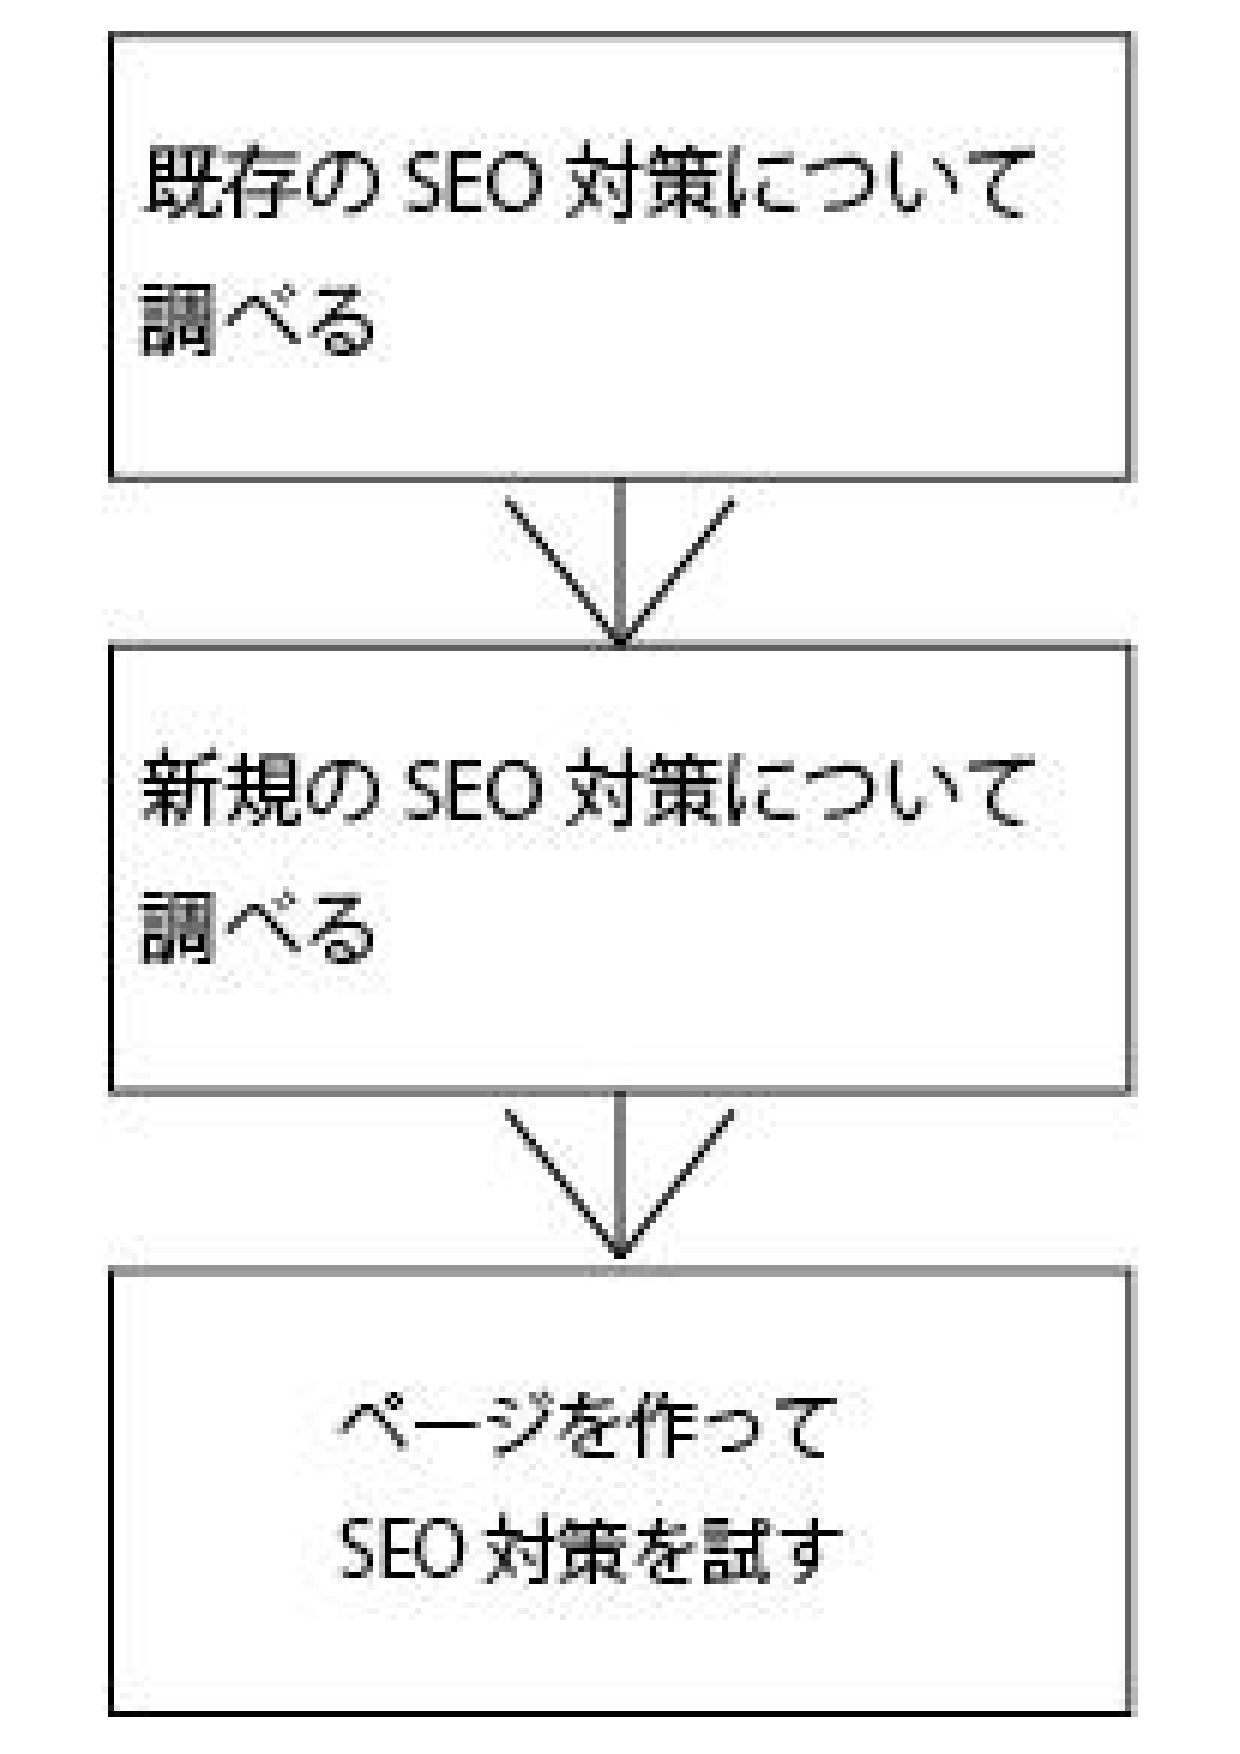
\includegraphics[width=5cm,clip]{images.pdf}
\caption{図は\texttt{主な}作業の流れである.}\label{サンプル図}
\end{wrapfigure}

研究方法としてまず初めに既存のSEO対策について調べる.
既存のSEO対策として相対リンクや被リンクの数,ページの構成,データの有益性,検索されたワードがどのくらい入っているか等がある.この他にもあるSEO対策について調べサイトを上位に上げる必要事項をリスト化していく.


%\begin{wraptable}[行数]{r}{幅}%行数はオプションだが,調整しないとうまくいかない.
\begin{wraptable}[8]{r}{4cm}
\vspace*{-\intextsep}

\begin{tabular}{cc}
\hline

\hline
\end{tabular}
\end{wraptable}

次に検索上位に表示されるページの傾向について調べる.そしてそこから検索上位に表示される為の必要事項が見つかった場合リストに追加していく.



\par

この既存のSEO対策がどのくらい効果があるか調べるため自分でサイトを作り実際に検索結果に効果があるか調べる.\par
例に挙げたSEO対策の実践方法としては以下を行う予定である.\par
・リンクはブログやサイトなどを運営して相対リンク,被リンクを行う.そのほかに相対リンクを行ってくれるサイト等を活用する.\par
・ページの構成はテンプレートを使う,自分でHTMLを書くなどして構成を変える.\par
・データの有益性についてはについては目下調査中.\par
・キーワードについてはテキストやmetaタグに入れるなどして増やしていく.
\newpage
\section{現在の進捗状況}
既存のSEO対策について調査中.
\section{今後の計画}
・一般的なSEO対策について調べる\par
・上位サイトの関連性について調べる\par
・サイトを作る\par

書籍\cite{takano2016},

\bibliographystyle{junsrt}
\bibliography{biblio}%「biblio.bib」というファイルが必要.

\end{document}





